\documentclass[aspectratio=169]{beamer}
%
% Choose how your presentation looks.
%
% For more themes, color themes and font themes, see:
% http://deic.uab.es/~iblanes/beamer_gallery/index_by_theme.html
%
\mode<presentation>
{
  \usetheme{metropolis}      % or try Darmstadt, Madrid, Warsaw, ...
  \usecolortheme{metropolis-imagelab} % or try albatross, beaver, crane, ...
  \usefonttheme{structurebold}  % or try serif, structurebold, ...
  \setbeamercolor{background canvas}{bg=white}
  \setbeamertemplate{navigation symbols}{}
  \setbeamertemplate{bibliography item}{\insertbiblabel}
  %\setbeamertemplate{caption}[numbered]
} 
\usepackage[english]{babel}
\usepackage[utf8x]{inputenc}
\usepackage{algorithm,algorithmic}
\usepackage{listings}             % Include the listings-package
\usepackage{pgfplots}

\usepackage{tikz}
\usepackage{animate}
\usepackage{bm}


\hypersetup{
    colorlinks = true,
    linkcolor = {black},
    urlcolor = {blue}
}

\DeclareMathOperator*{\argmin}{arg\,min}
\DeclareMathOperator*{\argmax}{arg\,max}

\title[Logistic Regression and Gradient Descent]{Logistic Regression and Gradient Descent}
\subtitle{Pattern Recognition and Machine Learning}
\institute{University of Modena and Reggio Emilia}
\author{Davide Abati}
\date{October 19th, 2017}

\def\thisframelogos{}

\newcommand{\framelogo}[1]{\def\thisframelogos{#1}}

\begin{document}

\framelogo{logo_unimore_white.png}

\bgroup
\renewcommand{\insertframenumber}{}
\begin{frame}[noframenumbering]
  \titlepage
\end{frame}
\egroup
\bgroup
\begin{frame}{Supervised learning setting}
We are given a training set $\{X_i, Y_i\}_{i=1}^N$, with $X_i \in \mathbb{R}^m$ and $Y_i \in \{0, 1\}$ for each $i=1,\ldots,N$.
\begin{itemize}
\item $N$ is the number of training examples;
\item each example $X_i = \{x_i^{(1)}, \ldots , x_i^{(m)}\}$ is a vector of $m$ features;
\item each label $Y_i$ is either 0 or 1.
\end{itemize}
\end{frame}
\egroup
\bgroup
\begin{frame}{Logistic regression}
\only<1>{
We need to learn a function that maps X to Y such that ``it works well on the training set''.
}

\only<2>{
We need to learn the parameters $\textbf{w}$ of a parametric function that maps X to Y such that ``it works well on the training set''.
}

\only<3>{
We need to learn the parameters $\textbf{w}$ of a parametric function that maps X to Y such that \textbf{some error is as low as possible on the training set}.
}


\end{frame}
\egroup
\bgroup
\begin{frame}{Logistic regression classification rule}
The function for classification has the following form:
\begin{equation*}
F(X_i, w) = \sigma(w^T \cdot X_i), \quad \text{where} \quad \sigma(x) = \frac{1}{1+e^{-x}} = \frac{e^{x}}{1+e^{x}}
\end{equation*}
\begin{minipage}{0.45\textwidth}
\begin{itemize}
\onslide<2->{\item $\sigma(x)$ is called \textbf{sigmoid function};}
\onslide<3->{\item $w$ is a vector in $\mathbb{R}^m$, and is called \textbf{weight vector};}
\onslide<4->{\item $w$ is initialized randomly, but will improve as training goes.}
\end{itemize}
\end{minipage}
\onslide<2->{
\begin{minipage}{0.45\textwidth}
\begin{tikzpicture}
    \begin{axis}[
    	legend pos=north west,
        axis x line=middle,
        axis y line=left,
        x tick label style={/pgf/number format/fixed,
                            /pgf/number format/fixed zerofill,
                            /pgf/number format/precision=1},
        y tick label style={/pgf/number format/fixed,
                            /pgf/number format/fixed zerofill,
                            /pgf/number format/precision=1},
        %grid = major,
        width=7cm,
        height=4cm,
        grid style={dashed, gray!30},
        xmin=-4,     % start the diagram at this x-coordinate
        xmax= 4,    % end   the diagram at this x-coordinate
        ymin= 0,     % start the diagram at this y-coordinate
        ymax= 1,   % end   the diagram at this y-coordinate
        %axis background/.style={fill=white},
        xlabel=$w^T\cdot X_i$,
        ylabel=$\sigma(w^T\cdot X_i)$,
        tick align=outside,
        enlargelimits=false]
      % plot the stirling-formulae
      \addplot[domain=-5:5, blue, ultra thick,samples=500] {1/(1+exp(-x))};
    \end{axis}
\end{tikzpicture}
\end{minipage}
}
\end{frame}
\egroup
\bgroup
\begin{frame}{Binary crossentropy loss}
During training, we want to \textbf{minimize} the following function:
\begin{equation*}
\mathcal{L}(w) = -\frac{1}{N} \sum_{i=1}^N [Y_i \log(F(X_i, w)) + (1 - Y_i)\log(1-F(X_i, w))]
\end{equation*}
\end{frame}
\egroup
\setcounter{footnote}{0}
\begin{frame}{Gradient Descent\footnote{Credits for this slide: Andrea Palazzi \url{https://github.com/ndrplz/deep_learning_lectures}}}
\textbf{Gradient descent} is an iterative optimization algorithm for finding the minimum of a function. How? Take step proportional to the negative of the gradient of the function at the current point.
\begin{figure}
\begin{tabular}{c}
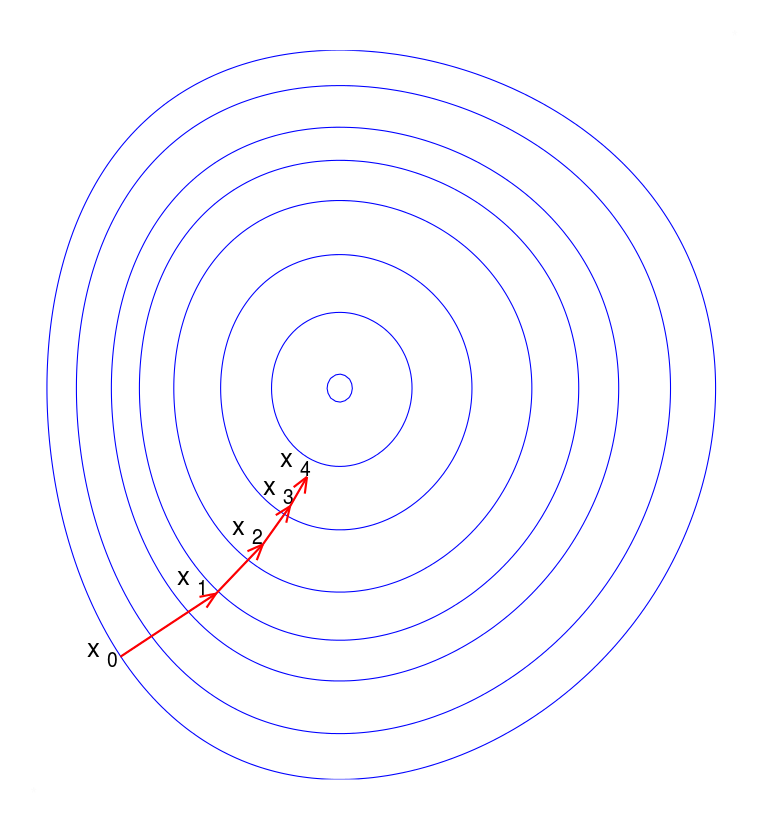
\includegraphics[width=0.2\textwidth]{img/sgd/level_sets.png}
\end{tabular}
\caption{Gradient descent on a series of level sets}
\end{figure}
\end{frame}

\setcounter{footnote}{0}
\begin{frame}{Gradient Descent Update\footnote{Credits for this slide: Andrea Palazzi \url{https://github.com/ndrplz/deep_learning_lectures}}}
If we consider a function $f(\bm{\theta})$, the \textbf{gradient descent update} can be expressed as:
\begin{equation}
\theta_j := \theta_j - \alpha \frac{\partial}{\partial \theta_j} f(\bm{\theta})
\end{equation}
for each parameter $\theta_j$.\\
\vspace{0.5cm}
The size of the step is controlled by \textbf{learning rate} $\alpha$.
\end{frame}

%%%%%%%%%%%%%%%%%%%%%%%%%%%%%%%%%%%%%%%%%%%%%%%%%%%%%%%%%%%%%%%%%%

%%%%%%%%%%%%%%%%%%%%%%%%%%%%%%%%%%%%%%%%%%%%%%%%%%%%%%%%%%%%%%%%%%
\setcounter{footnote}{0}
\begin{frame}{Visualizing Gradient Descent\footnote{Credits for this slide: Andrea Palazzi \url{https://github.com/ndrplz/deep_learning_lectures}}}
\begin{figure}
\begin{tabular}{c}
Gradient Descent for 1-d function $f(\theta)$.\\
  \animategraphics[loop,controls,width=0.9\textwidth]{1}{img/sgd/descent/descent-}{0}{7}
\end{tabular}
\end{figure}
\end{frame}


%%%%%%%%%%%%%%%%%%%%%%%%%%%%%%%%%%%%%%%%%%%%%%%%%%%%%%%%%%%%%%%%%%
\setcounter{footnote}{0}
\begin{frame}{Learning Rate\footnote{Credits for this slide: Andrea Palazzi \url{https://github.com/ndrplz/deep_learning_lectures}}}
Choosing the the right \textbf{learning rate} $\bm{\alpha}$ is essential to correctly proceed towards the minimum. A step \textit{too small} could lead to an extremely \textit{slow} convergence. If the step is \textit{too big} the optimizer could \textit{overshoot} the minimum or even \textit{diverge}. 
\begin{figure}
\begin{tabular}{ccc}
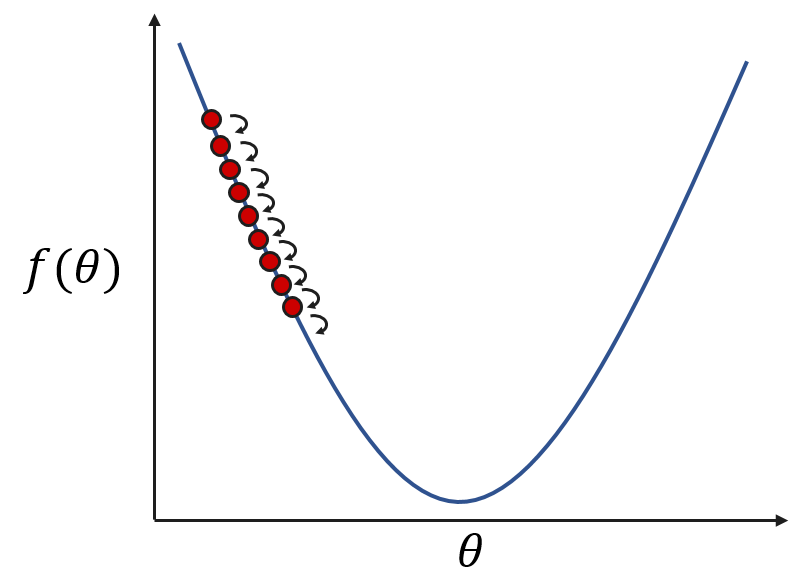
\includegraphics[width=0.35\textwidth]{img/sgd/lr_too_small.png} &
\quad &
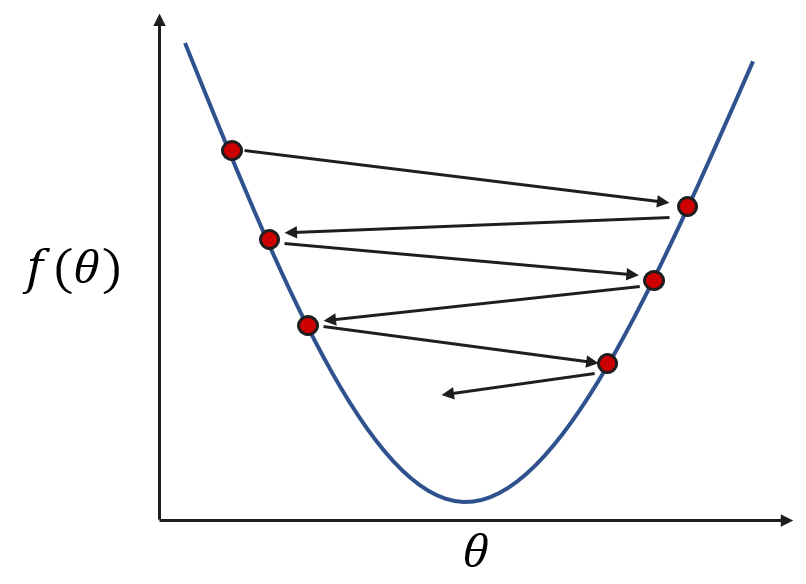
\includegraphics[width=0.35\textwidth]{img/sgd/lr_too_big.png}\\
Learning Rate too small & & Learning Rate too big
\end{tabular}
\end{figure}

\end{frame}

\bgroup
\begin{frame}{Simplify our loss}
Back to our problem. We need to take the derivative of this function w.r.t. $w$:
\begin{align*}
\mathcal{L}(w) &= -\frac{1}{N} \sum_{i=1}^N [Y_i \log(F(X_i, w)) + (1 - Y_i)\log(1-F(X_i, w))]\\
&=- \frac{1}{N} \sum_{i=1}^N \bigg[Y_i \log\bigg(\frac{e^{w^T\cdot X_i}}{1+e^{w^T\cdot X_i}}\bigg) + (1 - Y_i)\log\bigg(\frac{1}{1+e^{w^T\cdot X_i}}\bigg)\bigg]\\
&=- \frac{1}{N} \sum_{i=1}^N \bigg[Y_i(w^T\cdot X_i) - Y_i\log\bigg(1+e^{w^T\cdot X_i}\bigg) + (Y_i - 1)\log\bigg(1+e^{w^T\cdot X_i}\bigg)\bigg]\\
&=- \frac{1}{N} \sum_{i=1}^N \bigg[Y_i(w^T\cdot X_i) - \log\bigg(1+e^{w^T\cdot X_i}\bigg)\bigg]\\
\end{align*}
\end{frame}
\egroup
\bgroup
\begin{frame}{Derive the loss function}
Back to our problem. We need to take the derivative of this function w.r.t. $w$:
\begin{equation*}
\mathcal{L}(w) = -\frac{1}{N} \sum_{i=1}^N \bigg[Y_i(w^T\cdot X_i) - \log\bigg(1+e^{w^T\cdot X_i}\bigg)\bigg]
\end{equation*}
\begin{align*}
\frac{\delta \mathcal{L}(w)}{\delta w_j} &= -\frac{1}{N} \sum_{i=1}^N \bigg[Y_ix_i^{(j)} - \frac{e^{w^T\cdot X_i}}{1 + e^{w^T\cdot X_i}}x_i^{(j)}\bigg]\\
&=- \frac{1}{N} \sum_{i=1}^N \bigg[Y_i - \frac{e^{w^T\cdot X_i}}{1 + e^{w^T\cdot X_i}}\bigg]x_i^{(j)}\\
&=- \frac{1}{N} \sum_{i=1}^N \bigg[Y_i - F(X_i, w)\bigg]x_i^{(j)}
\end{align*}
\end{frame}
\egroup
\bgroup
\begin{frame}{Final gradient and update}
Back to our problem. We need to take the derivative of this function w.r.t. $w$:
\begin{align*}
\frac{\delta \mathcal{L}(w)}{\delta w} = \begin{bmatrix}
\frac{\delta \mathcal{L}(w)}{\delta w_1}\\[1em]
\frac{\delta \mathcal{L}(w)}{\delta w_2}\\[1em]
\vdots\\[1em]
\frac{\delta \mathcal{L}(w)}{\delta w_m}
\end{bmatrix} = 
\begin{bmatrix}
-\frac{1}{N} \sum_{i=1}^N (Y_i - F(X_i, w))x_i^{(1)}\\[1em]
-\frac{1}{N} \sum_{i=1}^N (Y_i - F(X_i, w))x_i^{(2)}\\[1em]
\vdots\\[1em]
-\frac{1}{N} \sum_{i=1}^N (Y_i - F(X_i, w))x_i^{(m)}
\end{bmatrix} = -\frac{X^T \cdot (Y-F(X,w))}{N}
\end{align*}
We will update the vector $w$ accordingly:
\begin{equation*}
w \leftarrow w - \alpha\frac{\delta \mathcal{L}(w)}{\delta w}
\end{equation*}
\end{frame}
\egroup
\bgroup  
\begin{frame}{Wrap up: algorithm}
\begin{algorithm}[H]
\begin{algorithmic}[1]
\STATE $X, Y \leftarrow load\_training\_data()$
\STATE set learning rate $\alpha$
\STATE initialize $w$ randomly
\FOR{$e=1$ to $number\_of\_training\_steps$}
\STATE compute the prediction according to the current weights $F(X, w)$
\STATE compute the loss function $\mathcal{L}(w)$
\STATE compute the derivative of the loss function w.r.t. weights $\frac{\delta \mathcal{L}(w)}{\delta w}$
\STATE update the weight vector $w \leftarrow w - \alpha\frac{\delta \mathcal{L}(w)}{\delta w}$
\ENDFOR
\end{algorithmic}
\caption{pseudocode for training}
\label{alg:train}
\end{algorithm}
\end{frame}
\egroup
\bgroup
\begin{frame}{Today's case study}
\begin{minipage}{0.45\textwidth}
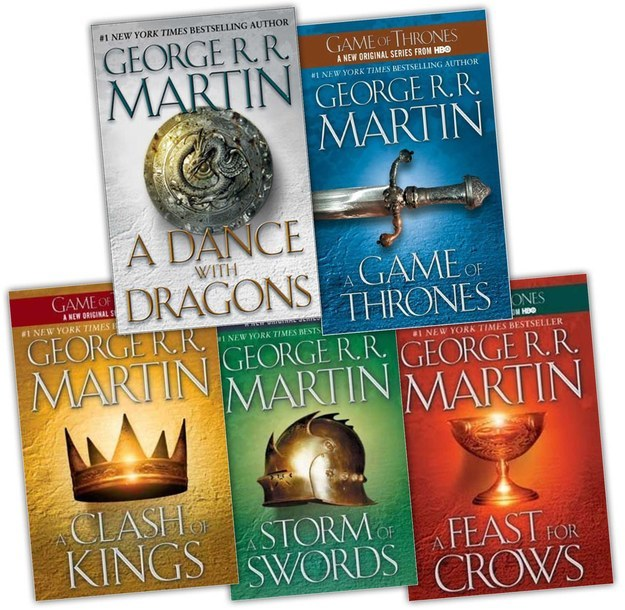
\includegraphics[width=\textwidth]{img/books.jpg}
\end{minipage}
\begin{minipage}{0.45\textwidth}
\begin{itemize}
\item We want to predict if a character is alive or dead;
\item (Some) of our features are:
\begin{itemize}
\item male or female; 
\item married or not;
\item number of deaths witnessed;
\item number of dead relatives;
\item ... and many more.
\end{itemize}
\end{itemize}
\end{minipage}
\end{frame}
\egroup

\end{document}